\section{Q3: Groupwise QUBO over Joint Candidate States}
\label{sec:q3-qubo}

\subsection{Groupwise formulation over the complete Q3 pool}

Question~3 minimizes the frozen candidate score over both the ordered
cation pair and the three permitted anion groups,
$\mathcal X_3=\{\mathrm{O}_3,\mathrm{NO}_2,\mathrm{FO}_2\}$.  File~08
contains $2,704$ candidates for each group, or 8,112 candidates in total.
We partition this complete domain by $X$ and construct three independent
104-variable models:
\begin{equation}
 (A_X^*,B_X^*)=
 \arg\min_{A,B\in\mathcal E}\widehat V_{23}(A,B,X),
 \qquad X\in\mathcal X_3.
 \label{eq:q3-group-objective}
\end{equation}
Each model has 52 A-site and 52 B-site one-hot variables and uses exactly
the integer cost and penalty construction in
Equations~\eqref{eq:q23-integer-cost}--\eqref{eq:q23-expanded-qubo}.  The
three models together cover every row of file~08 without projecting anion
identity into an approximate interaction.

The groupwise design also satisfies the adopted coefficient audit.
Each matrix contains only $-2$, 0, and 4, has an offset of 4, and maps to
integer Ising coefficients with $\max|h|=102$ and $\max|J|=1$.  With
$\lambda=2$, the minimum energy gap between an illegal state and the legal
minimum is two integer units in every group.

\subsection{Why QUBO energies are not compared across groups}

Although the three integer objectives use the same construction, they
do not share a common score origin.  In
Equation~\eqref{eq:q23-integer-cost}, the group minimum $m_X$ is subtracted
separately for each anion group before the remaining difference is capped
and rounded.  Each group winner therefore has an integer QUBO energy of
zero.  Those zero energies cannot be compared to decide which anion group
has the lowest original proxy score.

After decoding the best legal state returned for each group, the final
comparison therefore returns to the stored original-scale prediction:
\begin{equation}
 X^*=\arg\min_{X\in\mathcal X_3}
 \widehat V_{23}(A_X^*,B_X^*,X).
 \label{eq:q3-original-scale-comparison}
\end{equation}
This separation is important.  The QUBO energy selects a state within one
matrix, while $\widehat V_{23}$ compares decoded materials across matrices.
The integer energy is not an alternative physical metric.

\subsection{Matrix construction and enumeration audit}

For each group, we first enumerated the frozen file~08 predictions.
The generator then built the full $52\times52$ A--B interaction block and
archived the QUBO, offset, variable names, candidate identifiers,
legal-state index map, raw scores, and adapted Ising matrix.  Exhaustive
enumeration of the 2,704 legal states in each group identified a unique
minimum-energy state.  The formula, integer QUBO, and independently
recomputed discrete energies agreed exactly for all archived solver
samples.  Floating-point conversion audits are reported separately in
Section~\ref{sec:hardware-precision}.

On the original surrogate scale, the group minima were
Na--Nb--$\mathrm O_3$, Y--Ti--$\mathrm{NO}_2$, and
Na--Ti--$\mathrm{FO}_2$.  Their respective runners-up were
Sn--Ti--$\mathrm O_3$, Y--Zr--$\mathrm{NO}_2$, and
Sr--In--$\mathrm{FO}_2$, with margins of $0.013123$, $0.313819$, and
$0.028903$.  Each margin exceeds the $0.01$ threshold required by the
adopted two-level mapping to retain a unique zero-cost legal state.  These
are minima of the frozen proxy scores, not independently verified material
optima.  Because the Q2/Q3 pools are unlabeled, no independent error
estimate for $\widehat V_{23}$ is available; the margins therefore do not
establish statistically separated physical winners.

\subsection{CPU-local Kaiwu SDK results}

All three Q3 runs used the same Kaiwu SDK~1.4.3 CPU-local settings as
Q2: 30 seeds, up to ten returned samples per seed, 300 iterations per
temperature, and $\alpha=0.99$.  Table~\ref{tab:q3-sdk-results} reports
the decoded legal result on the original surrogate scale.  The time column
gives the recorded SDK wall time for each group.

\begin{table}[!htbp]
\centering
\caption{Groupwise Q3 results from the CPU-local Kaiwu SDK run.}
\label{tab:q3-sdk-results}
\small
\begin{tabularx}{\textwidth}{@{}lXrrrr@{}}
\toprule
$X$ & Best decoded candidate & $\widehat V_{23}$ & Legal/300 & Optimum seeds/30 & Time (s) \\
\midrule
O3  & Na--Nb--O3   & 0.540023 & 28 & 28 & 20.830 \\
NO2 & Y--Ti--NO2   & 1.491928 & 23 & 23 & 20.811 \\
FO2 & Na--Ti--FO2  & 0.878526 & 25 & 25 & 20.959 \\
\bottomrule
\end{tabularx}
\end{table}

Every legal sample returned within a group decoded to that group's
enumerated optimum.  The legal-sample fractions were $9.33\%$ for O3,
$7.67\%$ for NO2, and $8.33\%$ for FO2.  The corresponding group optimum
appeared in 28, 23, and 25 of the 30 SDK seeds.  Applying
Equation~\eqref{eq:q3-original-scale-comparison} selects candidate~4159,
Na--Nb--O3, with $\widehat V_{23}=0.5400229940675169$, equal to the
enumerated minimum in file~08.

\begin{figure}[!htbp]
\centering
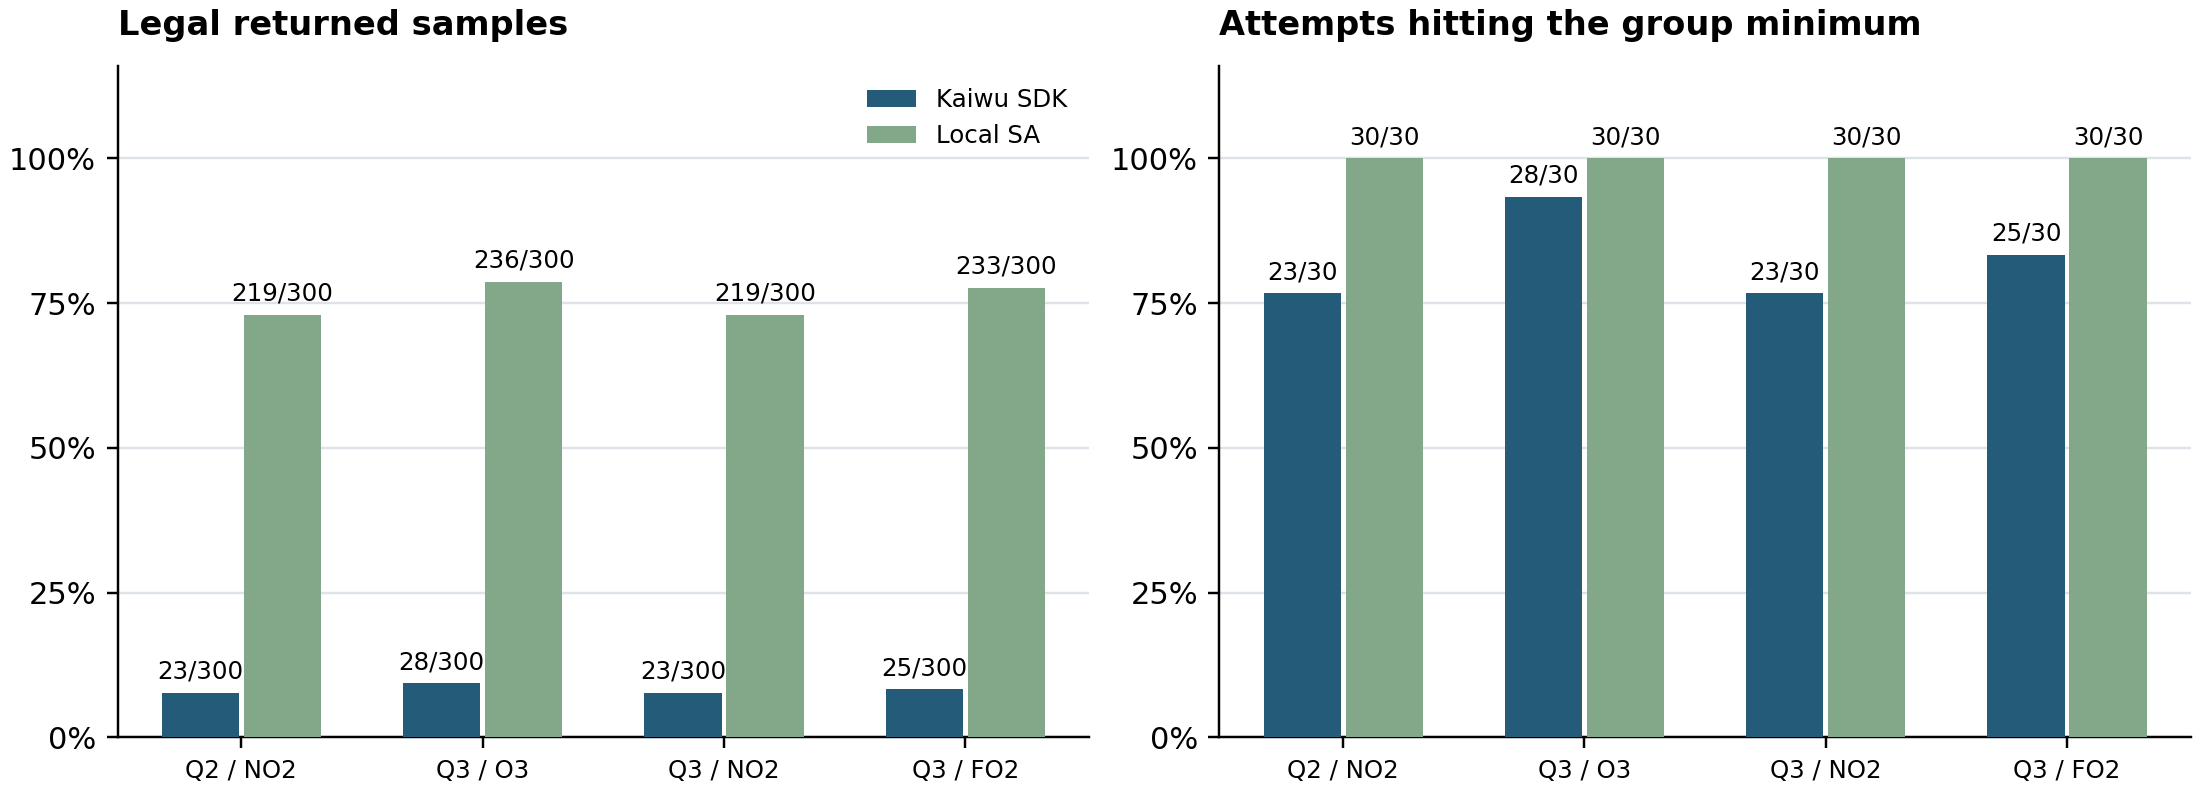
\includegraphics[width=\textwidth]{figures/q23_run_comparison.png}
\caption{Returned-sample quality for the adopted Q2 and Q3 matrices.  The
Kaiwu SDK bars use 30 independent SDK seeds with at most ten samples per
seed.  The local simulated-annealing comparison uses 300 chains divided
into 30 groups of ten, so an ``attempt'' has a different operational meaning
for the two backends.  The figure supports a sample-quality comparison only;
it does not establish a hardware speedup or quantum advantage.}
\label{fig:q23-run-comparison}
\end{figure}

Figure~\ref{fig:q23-run-comparison} also shows a separate local
simulated-annealing control.  That control returned more legal states and
hit every group optimum in all 30 chain groups.  Its implementation and
attempt definition differ from the SDK run, so the observed counts and wall
times are not used to claim a backend speed advantage.

\subsection{Comparison of 107-, 208-, and 104-variable encodings}

An alternative exact design represented the joint $(A,X)$ state with
$52\times3=156$ variables and B with 52 variables, producing one
208-variable floating-point QUBO.  The archived comparison verified all
8,112 legal-state energies against the original scaled costs with maximum
discrepancy zero.  Its SDK conversion produced 209 spins; after adding the
QUBO offset once, the corrected Ising constant was $K=13866.1509$ and the
maximum energy-chain residual was $4.57\times10^{-12}$.  Direct eight-bit
quantization did not preserve this model: the eight-bit rounding created
21--24 minimum ties, and sampled illegal states attained lower integer
energy than the best legal state.  It is therefore retained as an exact
floating-point and precision-stress comparison, not as the model used for
the reported Q3 solve.  The final groupwise method uses three 104-variable
matrices and performs the anion decision after decoding on the raw surrogate
scale.

The 107-variable control uses separate A, B, and X one-hot blocks with main,
A--B, A--X, and B--X terms.  It has no A--B--X interaction and fits a global
least-squares objective with ridge $10^{-8}$ over all 8,112 scores.  Its MAE,
RMSE, and Spearman correlation were 1.100009, 1.847176, and 0.978891, yet its
projected optimum was Rb--Ta--$\mathrm O_3$ (original-scale score 0.676651),
not Na--Nb--$\mathrm O_3$ (0.540023); Top-1 and Top-5 overlap were zero.
Because the low tail is a small part of the global loss, this model structure
is consistent with the observed winner change.  Without an interaction
ablation it is not established as the unique cause.

Table~\ref{tab:q3-encoding-comparison} aligns objective equivalence, oracle
dependence, variable count, coefficient range, ranking retention, legal-state
coverage, solve count, and role for the 107-, 208-, and 104-variable designs.
It is placed in the appendix to keep the main-text comparison compact.

\subsection{Evidence boundary and future work}

The Q3 result is limited to the frozen surrogate and the complete
file~08 candidate pool.  Na--Nb--O3 is the minimum identified by both
enumeration and the recorded solver samples under $\widehat V_{23}$; its
true violation score has not been measured.  We subsequently modeled
file~12 independently rather than filtering it after a full-pool solve.
Local simulated annealing on the dedicated floating-point and integer
104-variable blind matrices returned Ca--Sn--O3
($\widehat V_{23}=1.185082$), Y--Ti--NO2 (1.491928), and Rb--Ti--FO2
(1.590922).  All eight Q2/Q3 blind runs returned 300 of 300 legal samples.
For the integer matrices, fewer seed groups hit the optimum: 13 versus 27
for O3, 16 versus 25 for NO2, and 11 versus 26 for FO2.  This single
stochastic comparison does not establish integerization as the cause.
These are local-SA proxy results without blind physical labels, not SDK
or SPQC evidence.

Four final 104-variable matrices were submitted to SPQC-550.  The Q3/O3
task returned four legal samples out of ten, including the proxy winner
Na--Nb--O3.  The Q3/NO2 task returned no legal samples (0/7), while the
Q3/FO2 task returned one legal sample out of five, decoding to
Na--Ti--FO2.  Including Q2, three of the four tasks returned at least one
group proxy argmin, with unequal sample counts of 10, 10, 7, and 5.  This
task count is not an estimate of hardware success probability.  A separate
historical 30-variable task returned Ge--Ti--O3 and remains only a
reduced short-list comparison.  We therefore make no claim of physical
feasibility, hardware global optimality, speedup, or quantum advantage.
